\documentclass[12pt]{article}
\usepackage{fullpage,color}
\usepackage{amsmath,verbatim}
\usepackage{amssymb,amsthm}
\usepackage{amsmath,epsfig,fullpage,multirow}
\usepackage{graphicx}
\usepackage{subfigure}

\thispagestyle{empty}

\newcommand{\pa}{\partial}
\newcommand{\f}{\frac}


\begin{document}
\begin{center}
Math 505 --- HOMEWORK  \#7 a \hfill due Wednesday, October 29, 2014 (in class).\\
\hrule
\end{center}
\vskip 5pt

\noindent
In this homework we will study how to perform surface and line integrals on a general geometry.  

\flushleft
{\bf 1.} Find the mapping $H(r,s) = (H_1(r,s),H_2(r,s)) = (x,y)$ that, given the coordinates \mbox{$p_l, \, l = 1,2,3,4$}, maps the reference square $(r,s) \in [-1,1]^2$ into a straight-sided quad (see Figure \ref{fig:map}) in the $x-y$ plane. Hint: for each corner, find a bi-linear function that is one in one corner and zero in all other corners in the $r-s$ plane, and add them up. 

\begin{figure}[ht]
\begin{center}
\setlength{\unitlength}{1.0cm} 
\begin{picture}(8,5) 

\put(0,1.5){\vector(0,1){2}}
\put(0,1.5){\vector(1,0){2}}

\put(5.5,1.5){\vector(0,1){2}}
\put(5.5,1.5){\vector(1,0){2}}

\put(4.5,0.5){\color{blue}{\line(0,1){2}}}
\put(6.5,0.5){\color{blue}{\line(0,1){2}}}
\put(4.5,2.5){\color{blue}{\line(1,0){2}}}
\put(4.5,0.5){\color{blue}{\line(1,0){2}}}

\put(7.5,1.6){$r$}
\put(5.6,3.4){$s$}

\put(2.0,1.6){$x$}
\put(0.1,3.4){$y$}

\put(0.25,2.0){\color{blue}{\line(1,2){1}}}
\put(1.25,4){\color{blue}{\line(2,1){1}}}
\put(2.25,4.5){\color{blue}{\line(1,-3){0.615}}}
\put(0.25,2.0){\color{blue}{\line(4,1){2.61}}}


\put(0.1,1.7){$p_1$}
\put(2.9,2.5){$p_2$}
\put(2.1,4.7){$p_3$}
\put(0.8,4.0){$p_4$}

\put(4.1,0.4){$p'_1$}
\put(6.6,0.4){$p'_2$}
\put(4.1,2.4){$p'_4$}
\put(6.6,2.4){$p'_3$}


\end{picture}
\caption{\label{fig:map}}
\end{center}
\end{figure}


\flushleft
{\bf 2.} To compute integrals of the type $\iint f(x,y) dx dy $ we use the change of variables 
\[
x = H_1(r,s),\ \ y = H_2(r,s)),
\]
 and find that 
 \[
 \iint f(x,y) dx dy = \iint f(H_1(r,s),H_2(r,s)) | J | dr ds. 
 \]
 Here 
 \[
  | J | = \left| \left[  \begin{array}{cc}
  \frac{\partial x}{\partial r} & \frac{\partial x}{\partial s} \\
  \frac{\partial y}{\partial r} & \frac{\partial y}{\partial s}
   \end{array} \right] \right|.
  \]
Convince yourself that the formulas are correct by integrating (by repeated 1D quadrature, see chapter 5.4.2 in DQB) the area of a grid like the one displayed in Figure \ref{Fig:Grid}.
\begin{figure}[h]
  \begin{center}
  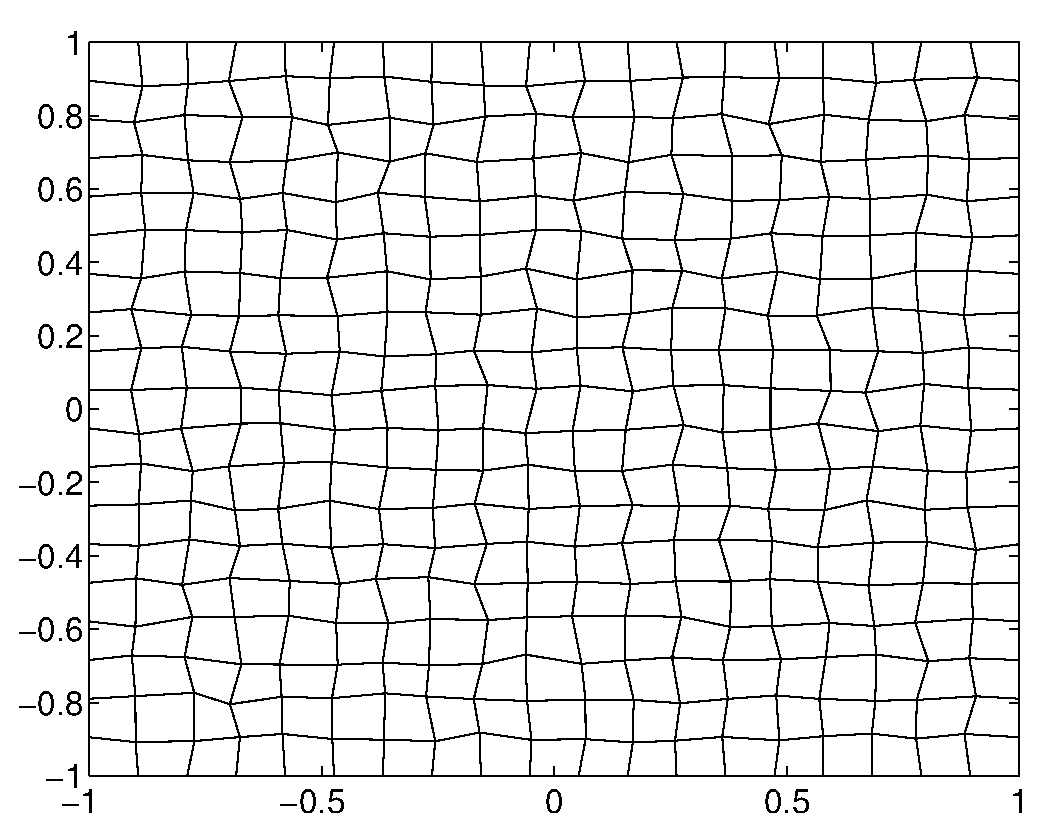
\includegraphics[width=0.5\textwidth]{grid}
  \caption{Grid made up of uniform Cartesian grid with the interior grid points randomly perturbed. \label{Fig:Grid}}
  \end{center}
\end{figure}
Report how the convergence depends on the quadrature for the 1D integrals, as well as on the total number of cells in the grid.

\flushleft
{\bf 3.} Use Green's identity and compute the same area by line integrals around each element. 

\flushleft
{\bf 4.} Also compute the area of the half annulus defined by the grid:
\begin{verbatim}
nr = 10; nt = 30; 
[r,theta] = meshgrid(linspace(0.5,1,nr),linspace(0,pi,nt));
x = r.*cos(theta); y = r.*sin(theta); 
plot(x,y,'k',x',y','k'), axis equal
\end{verbatim}

Why is it that the error converges as $\sim (\min (n_r,n_t))^{-2} $ independent of your choice of quadrature? 

In part b of this homework we will see how this can be fixed by the use of a slightly different mapping. 

\end{document}


















